\documentclass{article}
\usepackage{graphicx} % Required for inserting images

\title{N bidders}
\author{2200013213 }
\date{January 2024}

\begin{document}

\maketitle

\section{Introduction}
%N个工人,每个人被选中的权重为P_i(最终被选中的概率=P_i/提交块的人的P_i的和),每个人提交块的花费为A_i(可变),若被选中的收益函数为C_i(x),其中x为在块上的花费。
\par N workers, each one was selected with the probability function $P_i(x)$, with cost $A_i$, and profit function $C_i(x)$ . Everyone choose to compute the block with probability $Q_i$.
\subsection{Simplification 1: N=2 $A_1,A_2$ was fixed, $P_i(x)=P_i$ is fixed}
%工人只有两个,每个人提交块的花费固定,因此被选中的收益函数也固定
\par$E(income_1)=Q_1*(\frac{P_1}{P_2+P_1}Q_2*C(A_1)+(1-Q_2)C(A_1)-A_1)$
\par$E(income_1)=Q_1(-\frac{P_2}{P_2+P_1}Q_2*C(A_1)+C(A_1)-A_1)$
\par$E(income_2)=Q_2*(\frac{P_2}{P_2+P_1}Q_1*C(A_2)+(1-Q_1)C(A_2)-A_1)$
\par$E(income_2)=Q_2(-\frac{P_1}{P_2+P_1}Q_1*C(A_2)+C(A_2)-A_2)$
\par When $\frac{P_1}{P_2+P_1}<1-\frac{A_1}{C(A_1)}$, $E(income_1)>0$ always holds.
\par When $0>1-\frac{A_1}{C(A_1)}$, $E(income_1)<0$ always holds.

\begin{table}
    \centering


    \begin{tabular}{|c|l|c|c|} \hline 
  &$E(income_1)>0$& $E(income_1)?0$&$E(income_1)<0$\\ \hline 
          $E(income_2)>0$&$Q_1=1,Q_2=1$&$Q_1=0,Q_2=1$& $Q_1=0,Q_2=1$\\ \hline 
          $E(income_2)?0$&$Q_1=1,Q_2=0$&  Both $E$ =0& $Q_1=0,Q_2=1$\\ \hline 
          $E(income_2)<0$&$Q_1=1,Q_2=0$&  $Q_1=1,Q_2=0$& $Q_1=0,Q_2=0$\\ \hline
    \end{tabular}
    
    
\end{table}
Conclusion:
\par People have the motivation to cooperate when in the middle condition.($E(income_1)?0$ and $E(income_2)?0$)
\subsection{Simplification 2: $A_i$ was fixed, $P_i(x)=P_i$ is fixed}
\par Just as what we do in Simplification 1, We first write $E(income_i)=Q_i(-T_i*C(A_i)+C(A_i)-A_i)$, and $0<=T_i$, and $T_i$ doesn't contain $Q_i$. 
\par In fact $T_j=\sum_{X_i}(1-\frac{P_j}{P_j\sum_{X_i}P_i X_i})*\prod_{}Q_i^{X_i}X^{\sum_{X_i}P_i X_i}$ when $X=1$.
\par so $U^{'}(income_j)=\frac{\prod (1+Q_iX^{P_i})}{X}$ 
\par For at most $N$ loops, we find $i$ that either $E(income_i)>0$ or $E(income_i)<0$ . Then we get their best choice. And those left we concluded that they will have the motivation to cooperate.
\subsubsection{Note}\par If we $jinsi$ , that's say $T_j=1-\frac{P_j}{P_j+\sum Q_iP_i}$. It will be more efficient to compute.
\subsection{Simplification 3: N=2 ,$A_i$ has a boundary $B_i$, and $C_i(X)=C(X)$ is the same.}
\par We Suppose our $C(X)=\frac{M}{X}+S$ .
\par So $E(income_1)=(\frac{M}{A_1}+S)\frac{A_1}{A_1+A_2}-A_1$
 \par
 \begin{equation}
\begin{aligned}
&E^{'}(income_1)\ge 0
\\\Longleftrightarrow&\frac{A_2}{(A_1+A_2)^2}(\frac{M}{A_1}+S-A_1-A_2)\ge \frac{A_1}{A_1+A_2}(\frac{M}{A_1^2}+1)
\\\Longleftrightarrow&(A_1+A_2)^2-A_2S+M\le 0
\end{aligned}
\end{equation}
\par So if $A_2^2-SA_2+M\le 0$, Then $A_1=Min(-A_2+\sqrt{A_2S-M},B_1)$, else $A_1=0$
\par A good choice for both makes $E^{'}(income_1)=E^{'}(income_2)=0$, yields $A_1=A_2$, and $4A_1^2-A_1S+M=0$.
\par else we will stop at
\subsection{Simplification 3: N=2 ,$A_i$ has a boundary $B_i$, and $C_i(X)=C(X)$ is the same.}
\par we suppose $P_i(x)=A_i-b$.
So $E(income_1)=C(A_1)\frac{A_1-b}{A_1+A_2-2b}-A_1$
\subsubsection{Try 1:$C(X)=\frac{M}{X}+S$}
\par So $E(income_1)=(\frac{M}{A_1-b}+S)\frac{A_1-b}{A_1+A_2-2b}-A_1=\frac{M-\frac{b}{A_1}M-S}{A_1+A_2-2b}+\frac{A_1}{A_1+A_2-2b}(S-(A_1+A_2-2b))$
%讨论博弈平衡点时将A_i-b替换成A_i讨论
 \par
 \begin{equation}
\begin{aligned}
&E^{'}(income_1)\ge 0
\\\Longleftrightarrow&\frac{A_2}{(A_1+A_2)^2}(\frac{M}{A_1}+S-A_1-A_2)\ge \frac{A_1}{A_1+A_2}(\frac{M}{A_1^2}+1)
\\\Longleftrightarrow&(A_1+A_2)^2-A_2S+M\le 0
\end{aligned}
\end{equation}
\par So if $A_2^2-SA_2+M\le 0$, Then $A_1=Min(-A_2+\sqrt{A_2S-M},B_1)$, else $A_1=0$
\par A good choice for both makes $E^{'}(income_1)=E^{'}(income_2)=0$, yields $A_1=A_2$, and $4A_1^2-A_1S+M=0$.
%是否要给没成功的人一点补偿
%比如我们期望A_i=k_min b~k_max b, 我们让(1-1/k_min)M=S, 然后常数项最大值应该就是S/(k_min-1), 然后控制k_min来保证说常数项影响尽可能小。
\subsubsection{Try 2: $C(X)=\frac{MX}{X-b}$}
%可能需要控制一下进入条件,不然C(X)可能会太大。

\par So $E(income_1)=(\frac{MA_1}{A_1-b})\frac{A_1-b}{A_1+A_2-2b}-A_1=A_1(\frac{M}{A_1+A_2-2b}-1)$, is linear.
 \par
 \begin{equation}
\begin{aligned}
&E^{'}(income_1)\ge 0
\\\Longleftrightarrow&\frac{M}{(A_1+A_2-2b)}-1-A_1\frac{M}{(A_1+A_2-2b)^2}\ge 0
\\\Longleftrightarrow&(A_1+A_2-2b)^2-M(A_2-2b)\le 0
\\\Longleftrightarrow& b \le A_1 \le -(A_2-2b)+\sqrt{M(A_2-2b)}
\end{aligned}
\end{equation}
 \subsubsection{Try 3: $C(X)=\frac{MX}{P(X)}$}
%可能需要控制一下进入条件,不然C(X)可能会太大。
\par So $E(income_1)=(\frac{MA_1}{P(A_1)})\frac{P(A_1)}{\sum P(A_i)}-A_1=A_1(\frac{M}{\sum P(A_i)}-1)$, is linear.
 \par
 \begin{equation}
\begin{aligned}
&E^{'}(income_1)\ge 0
\\\Longleftrightarrow&\frac{M}{\sum P(A_i)}-1-A_1\frac{MP^{'}(A_1)}{(\sum P(A_i))^2}\ge 0
\\\Longleftrightarrow&(\sum P(A_i))^2-M(\sum P(A_i))+MA_1P^{'}(A_1)\le 0
\end{aligned}
\end{equation}
\subsubsection{Try 3: Add loser income}
%可能需要控制一下进入条件,不然C(X)可能会太大。
\par So $E(income_1)=C(X)\frac{P(A_1)}{\sum P(A_i)}+T\frac{P(A_1)}{\sum P(A_i)}-A_1=A_1(\frac{M}{\sum P(A_i)}-1)$, is linear.
 \par
 \begin{equation}
\begin{aligned}
&E^{'}(income_1)\ge 0
\\\Longleftrightarrow&\frac{M}{\sum P(A_i)}-1-A_1\frac{MP^{'}(A_1)}{(\sum P(A_i))^2}\ge 0
\\\Longleftrightarrow&(\sum P(A_i))^2-M(\sum P(A_i))+MA_1P^{'}(A_1)\le 0
\end{aligned}
\end{equation}

\section{2024/1/24}
%2024/1/24 To solve
%Scroll ,ZK_rollup的奖励
%Scroll 区块生成暂时由中心化机构负责
%polygon 与待合并的交易总数有关系,每一个交易打包是一样的。采用的是POS验证者竞争。
\href{https://eips.ethereum.org/EIPS/eip-225}{EIP-225:Clique 权威证明共识协议 (ethereum.org)}  
%stupid miner?合作/不合作的比例
\subsection{Baseline 1: polygon POS }
\par simplification:
\par miner's gets several kinds of income: fixed income( decided by the stake ) and dynamic income(from producing the block)
So $E(income_1)=C_0\frac{A_1}{\sum A_i}+\frac{C_1(A_1)}{\sum A_i}$
the $Ratio_1=\frac{E(income_1+income_2)}{E(income_1)+E(income_2)}=\frac{C_0(A_1+A_2)+C_1(A_1+A_2)}{C_0(A_1+A_2)+C_1(A_1)+C(A_1+A_2)}$
%Hard to deal with.It may decide by the algorithm and their protocol

\subsection{Baseline 2: fixed transactions fee and fixed Time}
%诚实矿工越多,聪明人挣得越多,聪明人特别多与特别少都有合作的欲望。(聪明人特别有钱)
%(聪明人特别没钱)诚实矿工越多,聪明人挣得越多;然而,聪明人增多,合作的欲望上升,聪明人再增多,合作欲望下降。分界线是两人资产和达到聪明人标准。
We have computed that \par So $E(income_1)=(\frac{M}{A_1-b}+S)\frac{A_1-b}{A_1+A_2-2b}-A_1$
We use $B_i=A_i-b$ ,and the limit $D_i$
We have $E(income_1)=(\frac{M}{B_1}+S)\frac{B_1}{B_1+B_2+\sum B_i}-B_1-b$
$E^{'}(income_1)\ge 0
\Longleftrightarrow(B_1+B_2+\sum B_i)^2-(B_2+\sum B_i)S+M\le 0$
$(0,-(B_2+\sum B_i)+\sqrt{(B_2+\sum B_i)S-M}$) increases
Suppose We have $N_0$ clever miners and $N_1$ stupid miners and 2 special miner.
That's to see what would happen
When 2 special miner work respectively, We suppose $N_0$ clever miners will not fulfill, otherwise it works just like stupid miner.
So the $B_{special1}=B_{special2}$ satisfy that $(N_0+2)^2X^2+(2C(N_0+2)-(N_0+1)S)X+C^2-SC+M=0$
So $2(N_0+2)X^2dN_0+2(N_0+2)^2XdX+(2C(N_0+2)-(N_0+1)S)dX+2CXdN_0=0$
So $dX=-X\frac{2(N_0+2)X+2C}{2(N_0+2)^2X+(2C(N_0+2)-(N_0+1)S)}$
$E(income_1)=(\frac{M}{X}+S)\frac{X}{(N_0+2)X+C}-X=\frac{M}{(N_0+2)X+C}+X(\frac{S}{(N_0+2)X+C}-1)$
$=\frac{M}{(N_0+2)X+C}+\frac{(N_0+2)M+S((N_0+2)X+C)^2}{(N_0+2)^2((N_0+2)X+C)^2}$
%C和(N_0+2)X总体是一比一负关系
%当N_0很大
\par1)When both are not fulfill
When $N_0+2->N_0+1$,$(N_0+2)X+C$ decrease a little($\frac{1}{(N_0+2)^2}$),$X$ increase a little($\frac{1}{(N_0+2)}$).
\par So $E(income_{1+2})=(1+\frac{4}{N_0+2})E(income_1)$
\begin{figure}
    \centering
    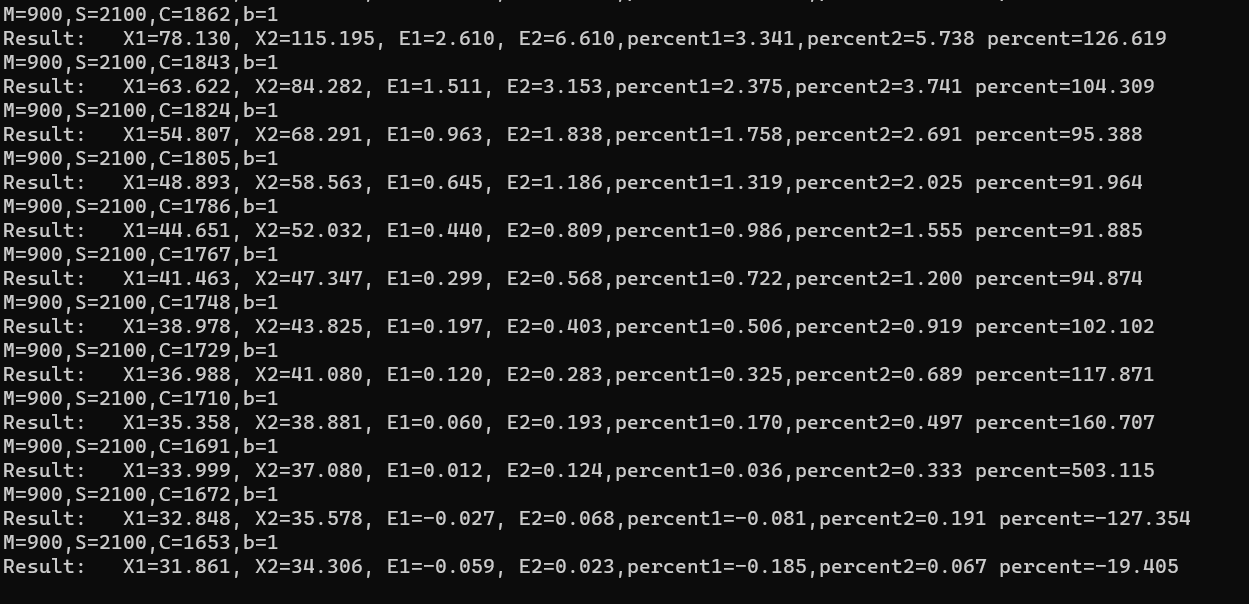
\includegraphics[width=1\linewidth]{3.png}
    \caption{Enter Caption}
    \label{fig:enter-label}
\end{figure}
\par2)When both are not fulfill
We can just think $\frac{E(income_{1+2})}{E(income_1)+E(income_2)}=\frac{(\frac{S}{SUM}-1)(B_1+B_2)+\frac{M}{SUM}-b}{(\frac{S}{SUM}-1)(B_1+B_2)+2(\frac{M}{SUM}-b)}$
%参考polygon,6000dollar/1年,取b=1(每天每人)B_average=19,B_SUM=2000,(100人),S为固定收益,100亿*5*1%*1/365=137万,(S+M)=137万,按照白皮书4%~5%收益率,我们认为大概有4000个链,所以S+M=3000.所以收益率为
%S=3000,M=0(bench) (B_1+B_2-2)/(B_1+B_2-4)=105.88%
%S=2500,   M=500                     102.8%
%S=2000,M=1000                       100%
%S=1000,M=2000                      93.2%
%最终取S=2100,M=900,期望收益每人每天为1.47368dollars,7.36847%
\begin{figure}
    \centering
    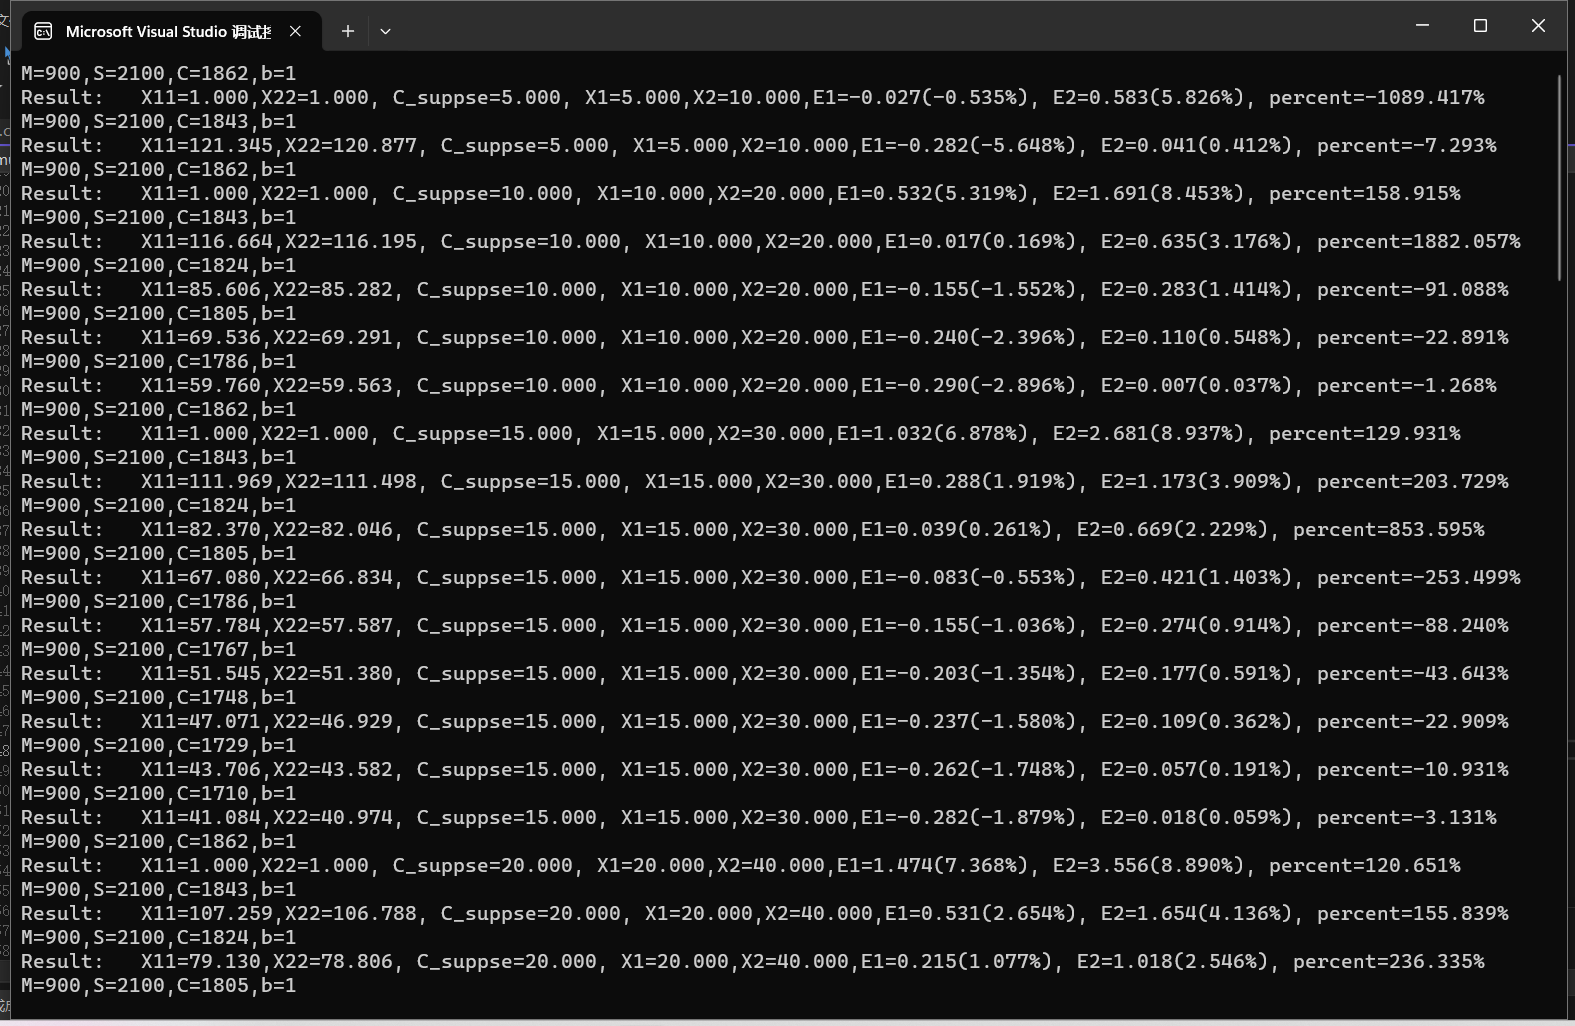
\includegraphics[width=1\linewidth]{2.png}
    \caption{Enter Caption}
    \label{fig:enter-label}
\end{figure}
%当N_0很小,视为0
Then when they do not cooperate
 $4X^2+(4C-S)X+C^2-SC+M=0$
 $(2X+(C-\frac{S}{4}))^2=M+\frac{S^2}{16}+\frac{SC}{2}$
 When they cooperate
  $(X+C)^2=(CS-M)$
\par1)When both are not fulfill
$E(income_1)=E(income_2)=(\frac{M}{X}+S)\frac{X}{2X+C}-X-b$
$E(income_{1+2})=(\frac{M}{x^{'}}+S)\frac{X^{'}}{X^{'}+C}-X^{'}-b$

\begin{figure}
    \centering
    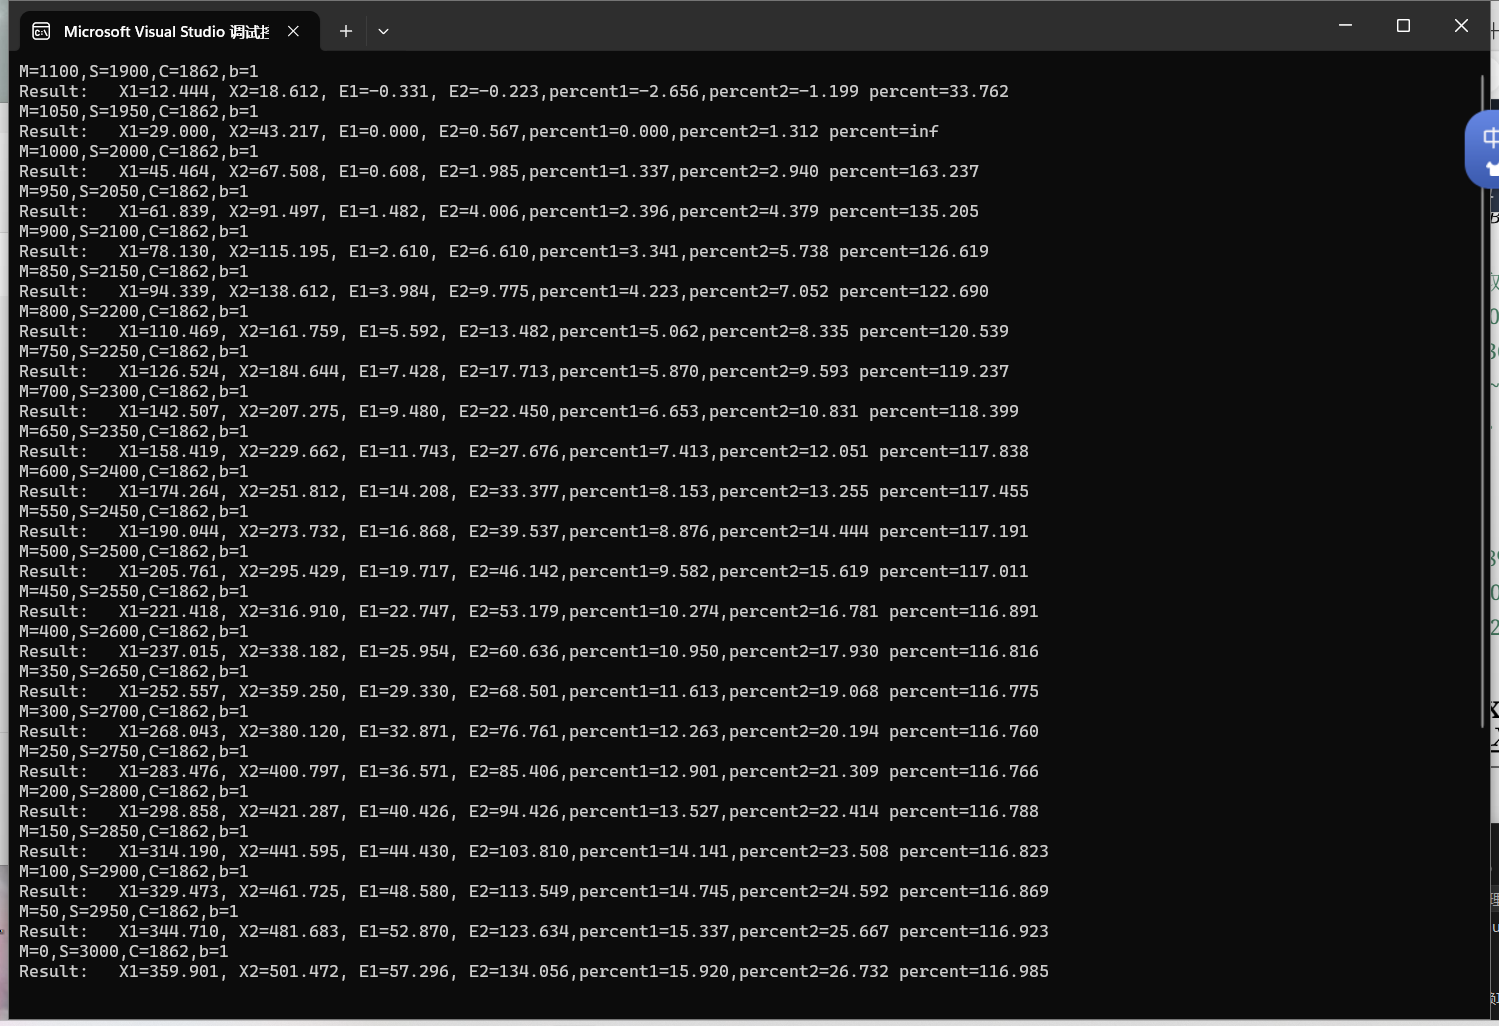
\includegraphics[width=1\linewidth]{1.png}
    \caption{Enter Caption}
    \label{fig:enter-label}
\end{figure}
\par2)When both are not fulfill
We can just think $\frac{E(income_{1+2})}{E(income_1)+E(income_2)}=\frac{(\frac{S}{SUM}-1)(B_1+B_2)+\frac{M}{SUM}-b}{(\frac{S}{SUM}-1)(B_1+B_2)+2(\frac{M}{SUM}-b)}$
%参考polygon,6000dollar/1年,取b=1(每天每人)B_average=19,B_SUM=2000,(100人),S为固定收益,100亿*5*1%*1/365=137万,(S+M)=137万,按照白皮书4%~5%收益率,我们认为大概有4000个链,所以S+M=3000.所以收益率为
%S=3000,M=0(bench) (B_1+B_2-2)/(B_1+B_2-4)=105.88%
%S=2500,   M=500                     102.8%
%S=2000,M=1000                       100%
%S=1000,M=2000                      93.2%
\begin{figure}
    \centering
    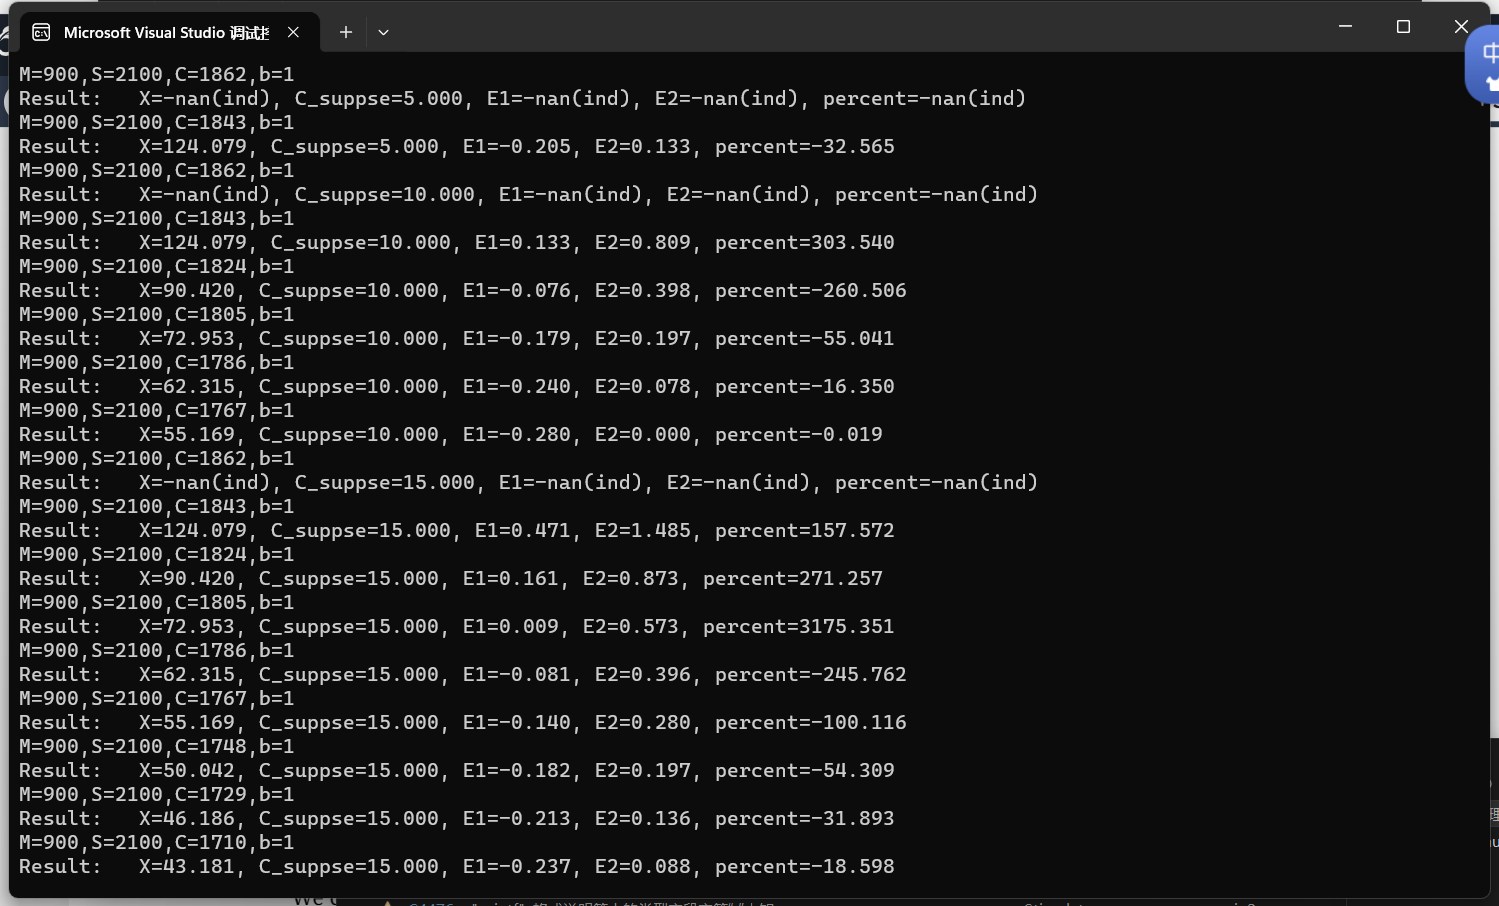
\includegraphics[width=1\linewidth]{4.png}
    \caption{Enter Caption}
    \label{fig:enter-label}

\end{figure}
\begin{figure}
    \centering
    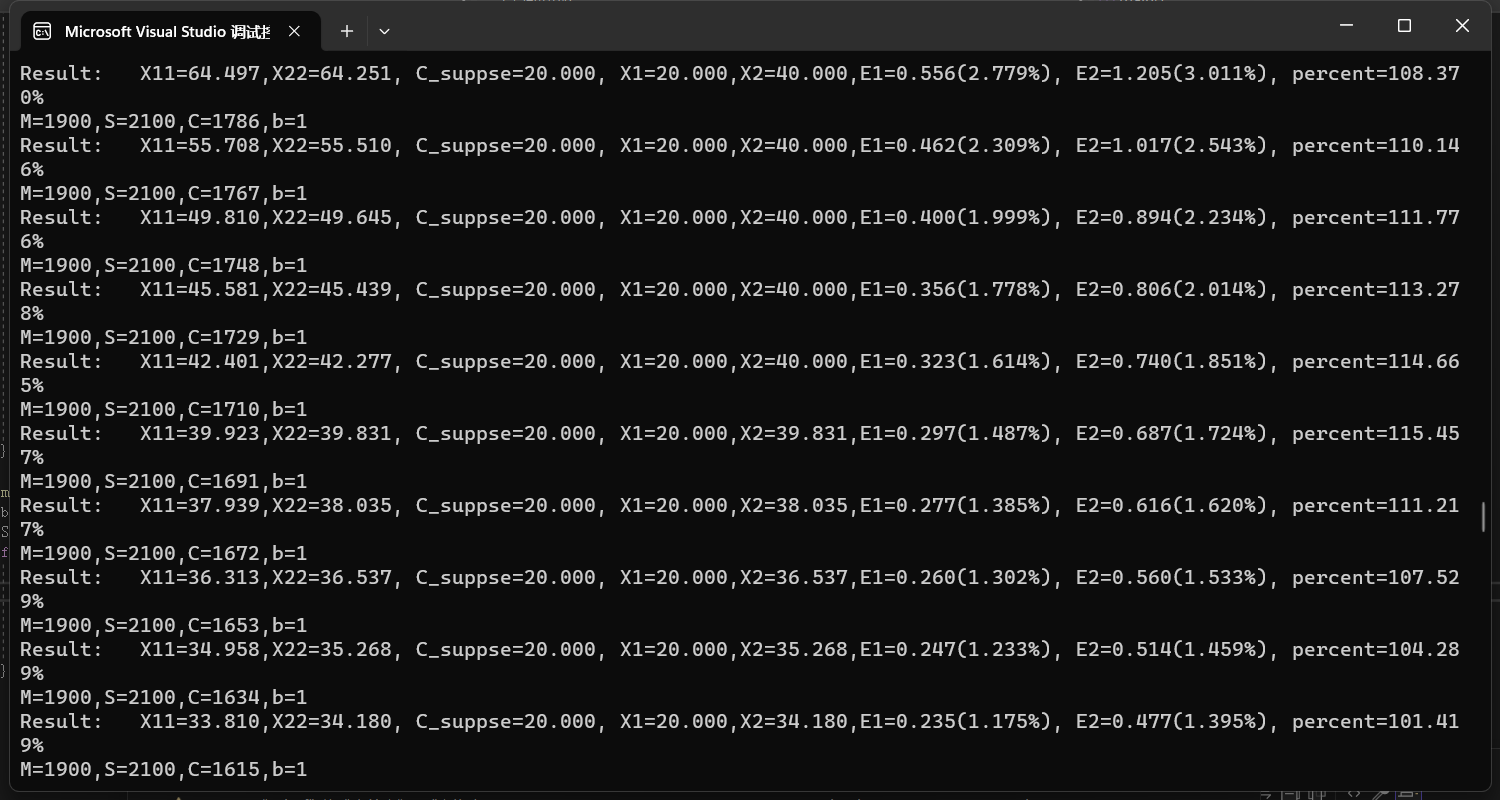
\includegraphics[width=1\linewidth]{7.png}
    \caption{Enter Caption}
    \label{fig:enter-label}
\end{figure}
\subsection{Baseline 3: fixed transactions fee and fixed Time With $C(X)=\frac{MX}{X-b}$}
We have computed that
\par So $E(income_1)=A_1(\frac{M}{\sum B_i}-1)$, is linear.
 \par
 \begin{equation}
\begin{aligned}
&E^{'}(income_1)\ge 0
\\\Longleftrightarrow&\frac{M}{B_1+\sum B_i}-1-A_1\frac{M}{(B_1+\sum B_i)^2}\ge 0
\\\Longleftrightarrow& 0 \le B_1 \le -\sum B_i+\sqrt{M(\sum B_i-b)}
\end{aligned}
\end{equation}
\par Similarly, we have $((N_0+2)X)^2+2(N_0+2)X(C-\frac{M(N_0+1)}{2(N_0+2)})+(C-\frac{M}{2})^2=\frac{M^2}{4}-Mb$
%参考polygon,6000dollar/1年,取b=1(每天每人)B_average=19,B_SUM=2000,(100人)取M=
%最终取M=2040,期望收益每人每天为1.47368dollars(28/19),7.36847%
\begin{figure}
    \centering
    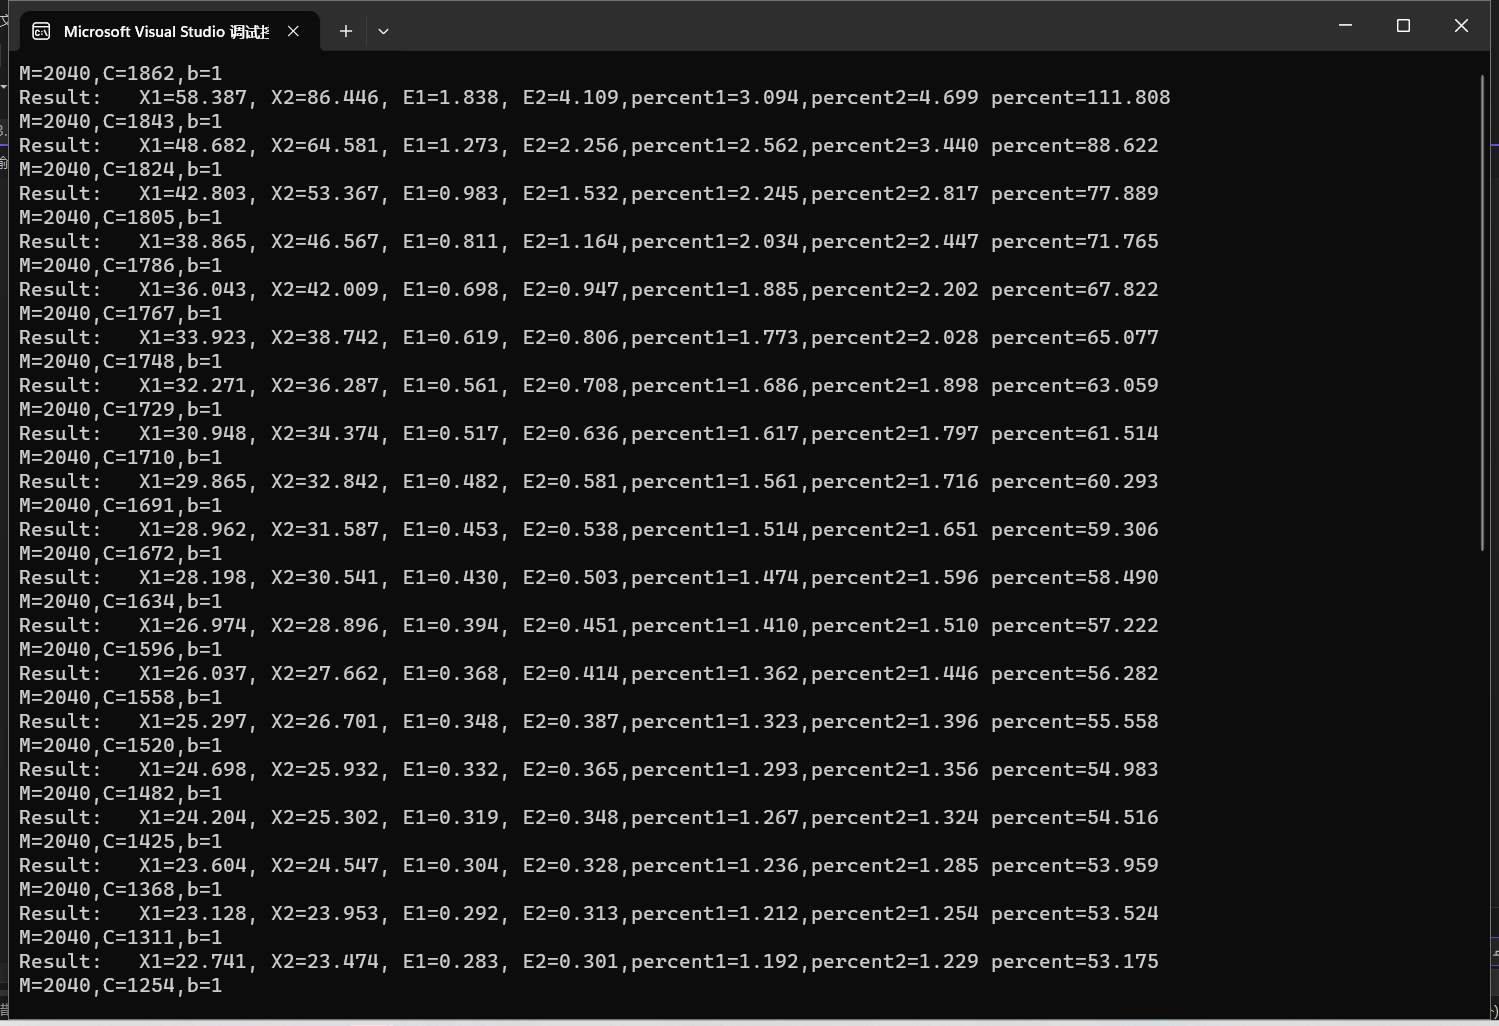
\includegraphics[width=1\linewidth]{5.png}
    \caption{Enter Caption}
    \label{fig:enter-label}
\end{figure}
\begin{figure}
    \centering
    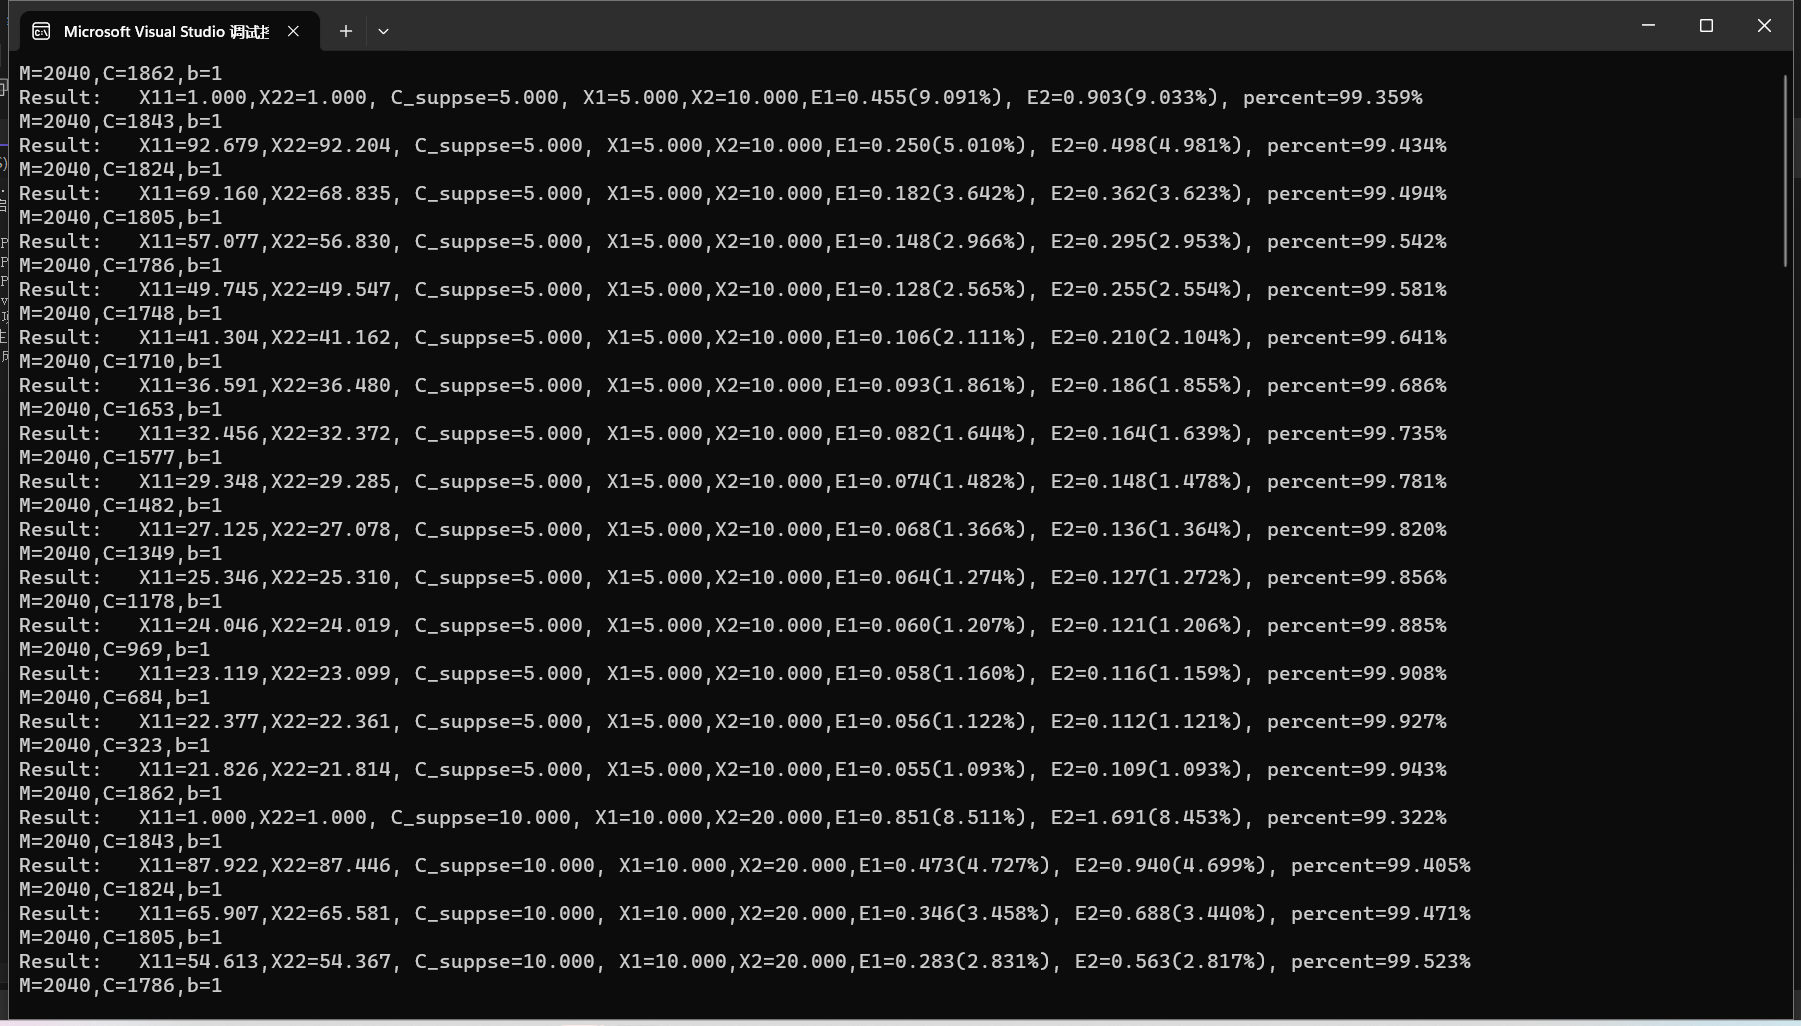
\includegraphics[width=1\linewidth]{6.png}
    \caption{Enter Caption}
    \label{fig:enter-label}
\end{figure}
%To solve:
%取值?
\end{document}


